% Options for packages loaded elsewhere
\PassOptionsToPackage{unicode}{hyperref}
\PassOptionsToPackage{hyphens}{url}
%
\documentclass[
  12pt,
]{article}
\usepackage{amsmath,amssymb}
\usepackage{lmodern}
\usepackage{setspace}
\usepackage{ifxetex,ifluatex}
\ifnum 0\ifxetex 1\fi\ifluatex 1\fi=0 % if pdftex
  \usepackage[T1]{fontenc}
  \usepackage[utf8]{inputenc}
  \usepackage{textcomp} % provide euro and other symbols
\else % if luatex or xetex
  \usepackage{unicode-math}
  \defaultfontfeatures{Scale=MatchLowercase}
  \defaultfontfeatures[\rmfamily]{Ligatures=TeX,Scale=1}
  \setmainfont[Scale=MatchLowercase]{Merriweather}
\fi
% Use upquote if available, for straight quotes in verbatim environments
\IfFileExists{upquote.sty}{\usepackage{upquote}}{}
\IfFileExists{microtype.sty}{% use microtype if available
  \usepackage[]{microtype}
  \UseMicrotypeSet[protrusion]{basicmath} % disable protrusion for tt fonts
}{}
\makeatletter
\@ifundefined{KOMAClassName}{% if non-KOMA class
  \IfFileExists{parskip.sty}{%
    \usepackage{parskip}
  }{% else
    \setlength{\parindent}{0pt}
    \setlength{\parskip}{6pt plus 2pt minus 1pt}}
}{% if KOMA class
  \KOMAoptions{parskip=half}}
\makeatother
\usepackage{xcolor}
\IfFileExists{xurl.sty}{\usepackage{xurl}}{} % add URL line breaks if available
\IfFileExists{bookmark.sty}{\usepackage{bookmark}}{\usepackage{hyperref}}
\hypersetup{
  pdftitle={Mixing Expert Opinions: Three Worked Examples},
  pdfauthor={Brian Weatherson},
  hidelinks,
  pdfcreator={LaTeX via pandoc}}
\urlstyle{same} % disable monospaced font for URLs
\usepackage[margin=1.38in]{geometry}
\usepackage{graphicx}
\makeatletter
\def\maxwidth{\ifdim\Gin@nat@width>\linewidth\linewidth\else\Gin@nat@width\fi}
\def\maxheight{\ifdim\Gin@nat@height>\textheight\textheight\else\Gin@nat@height\fi}
\makeatother
% Scale images if necessary, so that they will not overflow the page
% margins by default, and it is still possible to overwrite the defaults
% using explicit options in \includegraphics[width, height, ...]{}
\setkeys{Gin}{width=\maxwidth,height=\maxheight,keepaspectratio}
% Set default figure placement to htbp
\makeatletter
\def\fps@figure{htbp}
\makeatother
\setlength{\emergencystretch}{3em} % prevent overfull lines
\providecommand{\tightlist}{%
  \setlength{\itemsep}{0pt}\setlength{\parskip}{0pt}}
\setcounter{secnumdepth}{5}
\usepackage[italic]{mathastext}
\usepackage{booktabs}
\usepackage{longtable}
\usepackage{array}
\usepackage{multirow}
\usepackage{wrapfig}
\usepackage{float}
\usepackage{colortbl}
\usepackage{pdflscape}
\usepackage{tabu}
\usepackage{threeparttable}
\usepackage{threeparttablex}
\usepackage[normalem]{ulem}
\usepackage{makecell}
\usepackage{xcolor}
\ifluatex
  \usepackage{selnolig}  % disable illegal ligatures
\fi
\newlength{\cslhangindent}
\setlength{\cslhangindent}{1.5em}
\newlength{\csllabelwidth}
\setlength{\csllabelwidth}{3em}
\newenvironment{CSLReferences}[2] % #1 hanging-ident, #2 entry spacing
 {% don't indent paragraphs
  \setlength{\parindent}{0pt}
  % turn on hanging indent if param 1 is 1
  \ifodd #1 \everypar{\setlength{\hangindent}{\cslhangindent}}\ignorespaces\fi
  % set entry spacing
  \ifnum #2 > 0
  \setlength{\parskip}{#2\baselineskip}
  \fi
 }%
 {}
\usepackage{calc}
\newcommand{\CSLBlock}[1]{#1\hfill\break}
\newcommand{\CSLLeftMargin}[1]{\parbox[t]{\csllabelwidth}{#1}}
\newcommand{\CSLRightInline}[1]{\parbox[t]{\linewidth - \csllabelwidth}{#1}\break}
\newcommand{\CSLIndent}[1]{\hspace{\cslhangindent}#1}

\title{Mixing Expert Opinions: Three Worked Examples}
\author{Brian Weatherson}
\date{2021-01-30}

\begin{document}
\maketitle

\setstretch{1.1}
What should you do if two experts, each of whom you are disposed to
defer to, disagree? The answer depends on what you know about the
relationship between the experts' evidence. I'm going to argue for this
dependence claim, and work through three examples that start the process
of illustrating the nature of the dependence. The first example concerns
a case where the evidence the experts have is maximally independent.
This case has been well analysed by
\protect\hyperlink{ref-EaswaranEtAl2016}{Easwaran et al.}
(\protect\hyperlink{ref-EaswaranEtAl2016}{2016}), and my main
contribution is to offer a new (and perhaps more explanatory) proof of
their primary conclusion. The second case is where you know what
proportion of the experts' evidence is shared. And the third is where
you know that one expert is more informed, but you don't know which. In
each of the last two cases I'll show the computed exact values of the
posterior probabilities after conditionalising on the expert credences,
and also show some simple methods for approximating these exact values.
The approximations are, I suspect, a little more robust when we move
from the simple examples I'll describe to more realistic ones.

So let's get more precise about the question we're asking, and also give
names to the characters in the story. (It feels weird to talk about you
when I don't know who you are, so I prefer having named characters.)
Assume Player regards Ivy and Zack as experts about \(p\) in the
following sense.

\begin{enumerate}
\def\labelenumi{(\arabic{enumi})}
\tightlist
\item
  If Player learns that Ivy's credence in \(p\) is \(x\), and nothing
  else, he will change his credence in \(p\) to \(x\).
\item
  If Player learns that Zack's credence in \(p\) is \(x\), and nothing
  else, he will change his credence in \(p\) to \(x\).
\end{enumerate}

Given that, what is the answer to this question.

\begin{enumerate}
\def\labelenumi{(\arabic{enumi})}
\setcounter{enumi}{2}
\tightlist
\item
  If Player learns that Ivy's credence in \(p\) is \(y\), and Zack's
  credence in \(p\) is \(z\), and nothing else, what should his credence
  in \(p\) become?
\end{enumerate}

Following \protect\hyperlink{ref-BaccelliStewart2021}{Baccelli and
Stewart} (\protect\hyperlink{ref-BaccelliStewart2021}{2021}), let's
distinguish two kinds of answers to this question. The
\emph{supra-Bayesian} says that this case, like every other case, calls
for conditionalisation. This is going to be the kind of answer I defend.
Here's how we spell this answer out. First, we rewrite (1) and (2) as
(4) and (5)

\begin{enumerate}
\def\labelenumi{(\arabic{enumi})}
\setcounter{enumi}{3}
\tightlist
\item
  \(\forall x: Cr_P(p | Cr_I(p) = x) = x\)
\item
  \(\forall x: Cr_P(p | Cr_Z(p) = x) = x\)
\end{enumerate}

Where \(Cr_P, Cr_I\) and \(Cr_Z\) are Player, Ivy and Zack's credence
functions respectively. Then (3) gets rephrased as a request for the
value of

\begin{enumerate}
\def\labelenumi{(\arabic{enumi})}
\setcounter{enumi}{5}
\tightlist
\item
  \(Cr_P(p | Cr_I(p) = y \wedge Cr_I(p) = z)\)
\end{enumerate}

That's good as far as it goes, but it raises two natural questions.
First, what reasonable credal functions make (4) and (5) true, and what
do they tend to say about (6)? Second, given the massive computational
difficulty in calculating values like (6) in real time, are there
heuristics for approximating its value in realistic cases? This paper
aims to make progress on both questions. It offers some examples of
reasonable credal functions satisfying (4) and (5), and uses them to
suggest some heuristics for approximating (6) in somewhat realistic
cases.

But before we get to those answers, we should look at the other kind of
answer \protect\hyperlink{ref-BaccelliStewart2021}{Baccelli and Stewart}
(\protect\hyperlink{ref-BaccelliStewart2021}{2021}) mention: pooling
answers. A pooling answer to (3) says that we should find some function
that in some way `pools' \(y\) and \(z\) to answer (3). One obvious such
function is the arithmetic mean. The answer to (3) is just
\((y + z)/2\). Unfortunately, this won't do for three reasons. One
reason, as proven independently by
\protect\hyperlink{ref-Gallow2018}{Gallow}
(\protect\hyperlink{ref-Gallow2018}{2018}) and
\protect\hyperlink{ref-Bradley2017}{Bradley}
(\protect\hyperlink{ref-Bradley2017}{2017}) is that it is incompatible
with supra-Bayesianism. A second reason, as stressed by
\protect\hyperlink{ref-RussellEtAl2015}{Russell, Hawthorne, and Buchak}
(\protect\hyperlink{ref-RussellEtAl2015}{2015}), is that it is in cases
where Player defers to Ivy and Zack across a range of questions, this
answer is incompatible with Player, Ivy and Zack all updating on
external evidence by conditionalisation.\footnote{Note that
  supra-Bayesianism is the view that Player should update on expert
  testimony by conditionalisation. This objection does not assume
  supra-Bayesianism, but does assume that conditionalisation is the
  right rule for normal, non-testimonial, updating.} A third reason, as
stressed by \protect\hyperlink{ref-Levinstein2015}{Levinstein}
(\protect\hyperlink{ref-Levinstein2015}{2015}) and
\protect\hyperlink{ref-EaswaranEtAl2016}{Easwaran et al.}
(\protect\hyperlink{ref-EaswaranEtAl2016}{2016}) is that in some cases
the intuitively correct answer to (3) is not between \(y\) and \(z\).

The last of these reasons is most pressing. The natural response to the
first two reasons is to move to some other kind of pooling. Both
\protect\hyperlink{ref-RussellEtAl2015}{Russell, Hawthorne, and Buchak}
(\protect\hyperlink{ref-RussellEtAl2015}{2015}) and
\protect\hyperlink{ref-BaccelliStewart2021}{Baccelli and Stewart}
(\protect\hyperlink{ref-BaccelliStewart2021}{2021}) suggest that we
should use some kind of geometric pooling instead of linear pooling. In
this context, to use geometric pooling is to give an answer to (3)
something like\footnote{I say `something like' because you might want to
  allow some extra parameters in the answer if, for example, you want to
  give different weights to the two experts. That kind of detail won't
  matter to the argument here; we're just going to focus on cases where
  the experts are treated symmetrically.}

\[
\frac{\sqrt{yz}}{\sqrt{yz} + {\sqrt{(1-y)(1-z)}}}
\]

And that pooling function can be shown to avoid the first two reasons
for not using linear pooling. But it can't avoid the third, and that's
what I'm going to focus on here.

There are three somewhat distinct reasons you might use pooling to
answer (3).

First, you might use it as a replacement for supra-Bayesianism. I'm
going to argue that if you do this, you also have to give up on
Bayesianism across the board. Sometimes the recipient of expert opinion
can reliably infer the evidence behind the opinion reliably. In those
cases, regular Bayesianism implies that the recipient should update on
just that evidence. And that regular, not supra, Bayesian principle is
enough to dispose of pooling answers.

There are two more plausible uses for a pooling answer. Second, you
might use it as a constraint on supra-Bayesianism. You could argue that
if the values that (6) takes for various \(y, z\) do not look like some
kind of pooling function, that's evidence the prior \(Cr_P\) was
irrational to start with. And third, you might use it as an
approximation for supra-Bayesianism. It's a lot easier to calculate
linear or geometric means than to work out precisely the value of (6).
Both of the last two uses are intuitively very plausible. One of the
arguments of this paper is that they are, unfortunately, ultimately
untenable. There just isn't much use around here for pooling.

Pooling answers to (3) look a lot like conciliationist approaches to
peer disagreement. Indeed, the form of pooling that uses linear
averaging is sometimes thought to be a application of the Equal Weight
View (\protect\hyperlink{ref-Elga2007}{Elga 2007}). Supra-Bayesian
answers look like evidentialist approaches to peer disagreement. In
particular, they look a lot like the Total Evidence View
(\protect\hyperlink{ref-Lackey2010-LACWSW}{Lackey 2010}). I'm going to
use an even older motivation for them: the evidentialist approach to
testimony defended by Frank \protect\hyperlink{ref-Jackson1987}{Jackson}
(\protect\hyperlink{ref-Jackson1987}{1987}). On Jackson's view,
testimony that \(p\) is evidence that the speaker has evidence for
\(p\). The way to rationally update on it depends on what kind of
evidence you think the speaker is likely to have, given they've
concluded \(p\), and what you would (rationally) do with that evidence.
Typically, the answer is \emph{Conclude p}. Jackson argues that while
this is typical, it isn't always the right answer. And it fails to be
the right answer in just the cases you shouldn't accept the speaker's
testimony.

So to simplify here, I'm going to look at some cases where Player can
simply deduce, given one of the experts' credences, what their evidence
must have been. And then Player will update on that evidence. As we'll
see, different assumptions about how the evidence of the experts
interacts leads to different answers to (3).

Two quick notes. First, I'm only going to look at cases where the
experts are treated symmetrically. That's a restriction, but it's a
useful one for letting us see the range of cases. Second, I'm going to
be agreeing with \protect\hyperlink{ref-EaswaranEtAl2016}{Easwaran et
al.} (\protect\hyperlink{ref-EaswaranEtAl2016}{2016}) a lot, especially
in the first half of the paper. I'm ultimately going to consider some
different kinds of cases to what they consider - but that's a difference
in focus, not a difference in conclusions. (They look at a bunch of
kinds of cases that I won't consider as well; it's not like I'm going
strictly beyond their work.) This paper is intended as a complement to
theirs, not at all a substitute. But I think it's a valuable complement,
because I'll show how some very realistic cases require a generalisation
of their model, and make some suggestions for what that generalisation
should look like.

\hypertarget{case-one-conditionally-independent-evidence}{%
\section{Case One: Conditionally Independent
Evidence}\label{case-one-conditionally-independent-evidence}}

In our first case, the experts' evidence is as independent as possible.
Here's a story to think about how that could be. Carmen has an urn with
50 marbles, 25 black and 25 white. She draws one at random and marks it
with invisible ink. She has a scanner that can detect which marble is
marked, but no one else can tell it apart from the other marbles. Let
\(p\) be the proposition that the marked marble is white - that's what
we'll focus on from now on.

After selecting one marble to be marked, she puts together a jar
containing the marked marble and 9 other marbles drawn at random from
the urn. (I'll use `urn' for where Carmen keeps all the unused marbles,
and `jar' for what she constructs to show the experts.) She shows that
to one of the experts, let's say Ivy. She gets to inspect the jar, i.e.,
count how many marbles in it are white and black. She then reports to
Player, but crucially not to Zack, her credence in \(p\).

In this example, the next thing that happens is that Carmen takes the
jar back, removes the 9 unmarked marbles, puts them back in the urn, and
draws a new set of 9 marbles. (That set may overlap with the first set
of course.) She puts these 9 in the jar, along with the marked marble,
and shows the jar to Zack. He examines the jar, and reports to Player
his credence in \(p\).

Now in this case we can work out precisely how Player should update on
these two pieces of information. When one expert reports a credence of
\(x\) in \(p\), Player can infer that they saw \(10x\) white marbles.
After all, what the expert knows is just that the marked marble is
equally likely to be any of the marbles in the jar they see. So given
\(Cr_I(p) = y\) and \(Cr_Z(p) = z\), Player can infer how many white
marbles were in each jar. And he can work out the probability of each of
those jars turning up given \(p\) and given \(\neg p\). And that's
enough to plug into Bayes's Theorem to work out a posterior probability
for \(p\). When you do that, you get the following result.

\begin{enumerate}
\def\labelenumi{(\arabic{enumi})}
\setcounter{enumi}{6}
\tightlist
\item
  \(Cr_P(p | Cr_I(p) = y \wedge Cr_Z(p) = z) = \frac{yz}{yz + (1-y)(1-z)}\)
\end{enumerate}

I'm not going to work through the derivation of this, because it's a
straightforward consequence of something I will derive below. If you do
want to check it for yourself, the key input is that the probability of
drawing \(x\) white balls in \(t\) draws without replacement from an urn
with \(w\) white balls and \(b\) black balls is

\[
\frac{\binom{w}{x} \binom{b}{t-x}}{\binom{w+b}{t}}
\]

More importantly, (7) looks just like a special case of the central
formula (Upco) that \protect\hyperlink{ref-EaswaranEtAl2016}{Easwaran et
al.} (\protect\hyperlink{ref-EaswaranEtAl2016}{2016}) use. And that's
not surprising, since this case uses the same conditional independence
assumption that they make through much of their paper. To say that \(A\)
and \(B\) are conditionally independent given \(C\) is just to say that
\(\Pr(A \wedge B | C) = \Pr(A | C)\Pr(B | C)\). In this case, any pair
of claims about how many white balls are in the jars shown to Ivy and to
Zack are conditionally independent, both conditional on \(p\) and on
\(\neg p\).

The right hand side of (7) also looks a lot like the geometric means
described above. The big difference is that the square root signs have
disappeared. And that makes a difference, because it means the result
violates what \protect\hyperlink{ref-BaccelliStewart2021}{Baccelli and
Stewart} (\protect\hyperlink{ref-BaccelliStewart2021}{2021}) call
Unanimity. This principle requires that
\(Cr_P(p | Cr_I(p) = y \wedge Cr_I(p) = y) = y\). If (7) is true then
Unanimity is violated in every case except where \(y\) equals 0, 0.5 or
1. But this is bad news for Unanimity, because the case for (7) in this
case seems very strong. Player really knows how many white marbles were
in each jar, and it's just a bit of algebra to get from there to (7) via
conditionalisation. And it's very plausible that conditionalisation is
the right way to update on evidence about how many marbles are in a jar.
So any principle incompatible with (7) is false.

It turns out that varying how many marbles are in the urn Carmen starts
with does not change (7). But changing the ratio of white marbles to
black marbles in the urn does change the formula. If the proportion of
the initial urn that is white is \(r\), then the general result is

\begin{enumerate}
\def\labelenumi{(\arabic{enumi})}
\setcounter{enumi}{7}
\tightlist
\item
  \(Cr_P(p | Cr_I(p) = y \wedge Cr_I(p) = z) = \frac{yz(1-r)}{yz(1-r) + (1-y)(1-z)r}\)
\end{enumerate}

Again, this isn't a new result;
\protect\hyperlink{ref-EaswaranEtAl2016}{Easwaran et al.}
(\protect\hyperlink{ref-EaswaranEtAl2016}{2016, 27}) derive an even more
general formula from which this falls out as a special case. But my way
of deriving it is just different enough to be worth including.

Let \(I_x\) be the disjunction of all possible evidence propositions
that would lead Ivy to have credence \(x\) in \(p\). In this case
\(I_x\) is a simple proposition that there are \(10x\) white marbles in
the jar, but we don't need to assume that \(I_x\) will be anything like
that simple. Everything that follows about \(I_x\) also holds for
\(Z_x\), the disjunction of all possible evidence propositions that
would lead Ivy to have credence \(x\) in \(p\), but I won't repeat the
derivations. Since Player defers to Ivy, i.e., (4) is true, we have the
following proof. (All credences are Player's, so I'll drop the
subscripts.)

\begin{align*}
Cr(p | I_x) &= x &&\therefore \\
Cr(p \wedge I_x) &= x \cdot Cr(I_x) \\
 &= x (Cr(p \wedge I_x) + Cr(\neg p \wedge I_x)) &&\therefore \\
(1-x)Cr(p \wedge I_x) &= x \cdot Cr(\neg p \wedge I_x)) &&\therefore \\
Cr(\neg p \wedge I_x)) &= \frac{1-x}{x} Cr(p \wedge I_x) &&\therefore \\
Cr(I_x | \neg p) &= \frac{(1-x)Cr(p)}{x\cdot Cr(\neg p)}Cr(I_x | p)
\end{align*}

So we know the ratio of \(Cr(I_x | p)\) to \(Cr(I_x | \neg p)\). That
will become useful in what follows. Assuming evidentialism, what matters
for (6) is working out the value of \(Cr(p | I_y \wedge Z_z)\). But we
now know enough to do that.

\[
Cr(p | I_y \wedge Z_z) = \frac{Cr(p \wedge I_y \wedge Z_z)}{Cr(I_y \wedge Z_z)}
\]

Using the general fact that \(X\) is equivalent to
\((p \wedge X) \vee (\neg p \wedge X)\), and that Player's credences are
probabilistic, so his credence in an exclusive disjunction equals the
sum of the credence in the disjuncts, we know this equals.

\[
\frac{Cr(p \wedge I_y \wedge Z_z)}{Cr(p \wedge I_y \wedge Z_z) + Cr(\neg p \wedge I_y \wedge Z_z)}
\]

Since \(Cr(p \wedge X) = Cr(X | p)Cr(p)\), we can rewrite this as

\[
\frac{Cr(I_y \wedge Z_z | p) Cr(p)}{Cr(I_y \wedge Z_z | p)Cr(p) + Cr(I_y \wedge Z_z | \neg p)Cr(\neg p)}
\]

And since \(I_y\) and \(Z_z\) are independent given both \(p\) and
\(\neg p\), this becomes

\[
\frac{Cr(I_y| p) Cr(Z_z | p) Cr(p)}{Cr(I_y| p) Cr(Z_z | p) Cr(p) + Cr(I_y| \neg p) Cr(Z_z | \neg p) Cr(\neg p)}
\]

If we assume the initial value of \(Cr(p) = r\), and use the earlier
derived fact that \(Cr(I_x | \neg p) = \frac{(1-x)r}{x(1-r)}Cr(p)\) this
becomes

\[
\frac{Cr(I_y| p) Cr(Z_z | p)r}{Cr(I_y| p) Cr(Z_z | p)r + \frac{(1-y)r}{y(1-r)} Cr(I_y| p) \frac{(1-z)r}{z(1-r)} Cr(Z_z | p) (1-r)}
\] Now we can finally eliminate \(Cr(I_y| p) Cr(Z_z | p)r\) from the top
and bottom, so this becomes

\[
\frac{1}{1 + \frac{(1-y)(1-z)r}{yz(1-r)}}
\]

Or in other words

\[
\frac{yz(1-r)}{yz(1-r) + (1-y)(1-z)r}
\]

And that's the completely general result when the evidence the experts
has is conditionally independent of both \(p\) and \(\neg p\), and
Player starts with credence \(r\) in \(p\).

But this case is surely rare. Experts typically have some training in
common that isn't shared by non-experts. So their reasons for having a
credence in \(p\) that differs from our prior will not be completely
independent. \protect\hyperlink{ref-EaswaranEtAl2016}{Easwaran et al.}
(\protect\hyperlink{ref-EaswaranEtAl2016}{2016}) note that sometimes we
can adjust for the common evidence by conditionalising on the common
evidence to come up with a new `prior,' or perhaps I should say
`intermediate' credence, \(r\), then applying this formula. This is
slightly more general, but still not a lot. Part of what makes us
non-experts be non-experts is that we don't have this common training,
so we can't identify what's common between the experts. Let's see if we
can come up with a slightly more general case.

\hypertarget{case-two-common-marbles}{%
\section{Case Two: Common Marbles}\label{case-two-common-marbles}}

In our second case, Carmen once again has an urn with 50 marbles, 25
black and 25 white. She draws one at random and marks it with invisible
ink. She can tell which one this is, but no one else can. And \(p\) is
still the proposition that the marked marble is white - that's what
we'll focus on from now on. After selecting the marble to be marked, she
puts together a jar containing the marked marble and 9 other marbles
drawn at random from the urn. She shows that to one of the experts,
let's say Ivy. She gets to inspect the jar, i.e., count how many marbles
in it are white and black. She then reports to Player, but crucially not
to Zack, her credence in \(p\).

So far, it's just like the last case. But what happens next is
(possibly) different. In this case, Carmen removes \(m\) unmarked
marbles from the jar, puts them back in the urn, and draws a new set of
\(m\) marbles to put in the jar. It's all random, so this could include
some of the marbles she just removed. She shows the jar to Zack, he
inspects it, and reports his credence in \(p\) to Player. And,
crucially, player knows \(m\), the number of marbles that are in common
between the jars. So \(m\) is a measure of the independence of the
experts' opinions.

Once again, we can work out precisely what Player's credence should be
given \(m\), and the two credences. Unfortunately, it's just a long
formula that doesn't seem to reduce nicely. But if you've got a machine
that's good at calculating hypergeometric distributions, and you dear
reader are probably reading this paper on a machine that's good at
calculating hypergeometric distributions, it's not that hard to
calculate the values by brute force. I won't list all the values, there
are several hundred of them, but I'll present them graphically here.
(Note I'll leave off the case where one or other expert announces a
credence of 0 or 1; in that case Player knows whether \(p\) is true, so
the question of how to merge the credences is easy.)

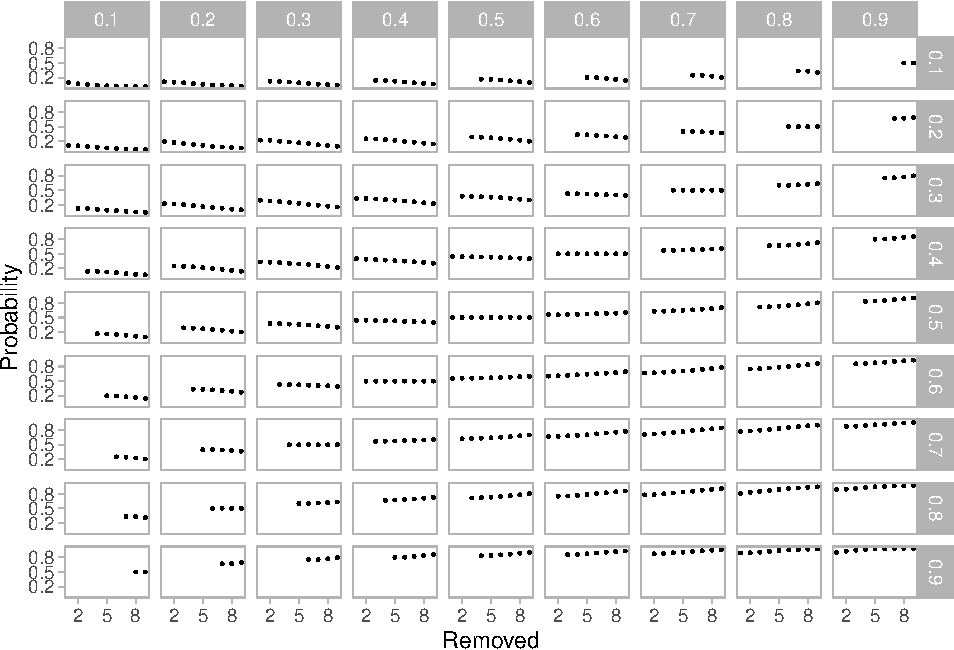
\includegraphics{mixing-experts-not-anon_files/figure-latex/unnamed-chunk-2-1.pdf}

Here is how to read the graph. Each row corresponds to a partiular
credence announced by Ivy; the credence is shown on the right. Each
column corresponds to a partiular credence announced by Zack; that
credence is shown on the top. The x-axis of the individual graphs shows
the value for \(m\), the number of marbles removed. And the y-axis shows
Player's final credence in \(p\). There are more dots on some graphs
than others because some combinations of Ivy credence, Zack credence and
\(m\) are impossible. The announced credences can't, by the rules of the
game, differ by more than \(0.1m\).

One notable feature of that graph is that as \(m\) gets larger, the
final credence tends to move away from 0.5; it tends to get more
opinionated. Another notable feature, though probably not one you can
see in this resolution, is that this move towards greater opinionation
happens in a surprisingly linear fashion. To a first approximation,
Player's credence moves away from 0.5 roughly the same amount for each
addition to \(m\), at least holding \(y\) and \(z\) fixed.

It's not perfectly linear, but it's much closer than I would have
guessed looking at how really quite non-linear the inputs are. Let's
zoom in on a part of the graph to see this more vividly.

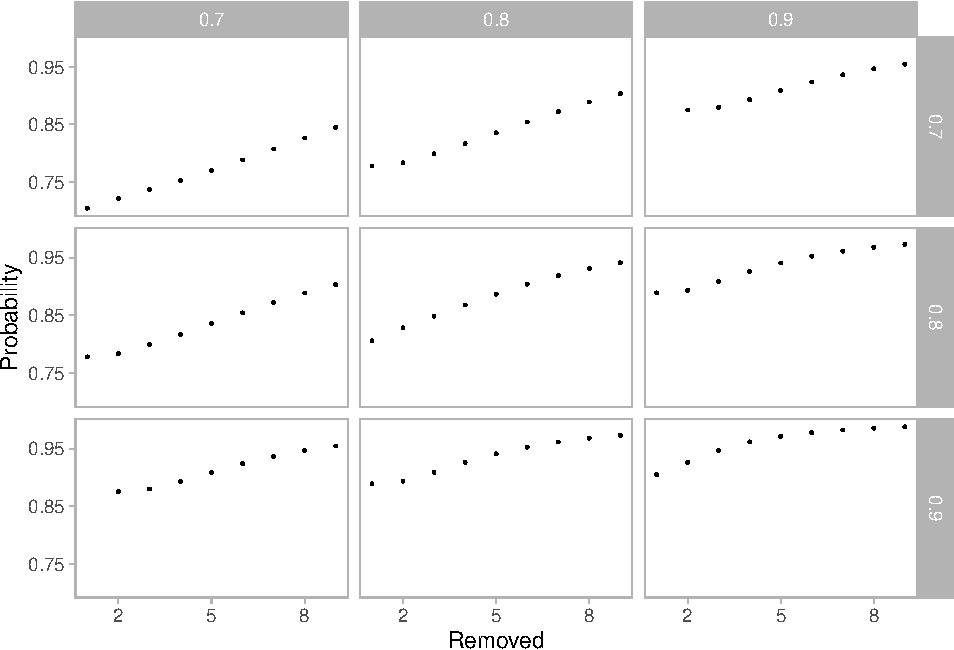
\includegraphics{mixing-experts-not-anon_files/figure-latex/unnamed-chunk-3-1.pdf}

The curve in the bottom right panel is not really linear; it definitely
curves downwards. But as you move your eye upwards and leftwards in the
table, the curves look much much straighter. The panel where they both
announce 0.7 is really remarkably straight. If we focus on the middle of
the big graph, this is even more striking. (I've left off the cases
where Zack announces a credence under 0.5 because those graphs are just
mirror images of graphs already shown.)

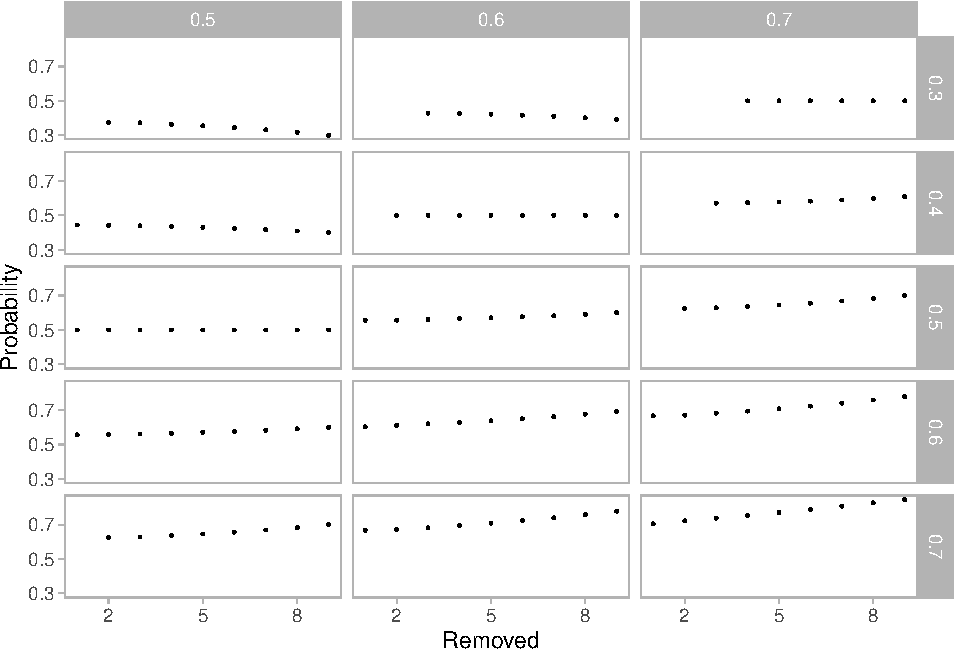
\includegraphics{mixing-experts-not-anon_files/figure-latex/unnamed-chunk-4-1.pdf}

Why does this matter? Because pooling functions are easy to use, and the
supra-Bayesian needs something to match that ease of use. It's a cliche
that for every problem there is a solution that is simple, intuitive,
and wrong. And the version of the pooling approach that uses linear
averages is very simple, very intuitive, and very wrong. The version
that uses geometric averages strikes most people as less simple and
intuitive (or maybe I'm just bad at explaining it), but it is less
wrong. But still, sometimes simple, intuitive and wrong is exactly what
you need! Computation is hard, life is short, precision is overrated.
Why not just average if you are just looking to get something roughly
right?

The supra-Bayesian can exploit the more-or-less linearity of the graphs
above graphs to come up with an approximation to these ideal Bayesian
credence. And the approximation isn't that much harder to calculate than
the geometric average. Intuitively, it works like this. If the experts
have exactly the same evidence, we take the geometric average of their
opinions.\footnote{We are working with cases so far where there is a
  unique rational credence for each evidence, so if they have the same
  evidence they have the same credence, and which kind of averaging we
  use is redundant. What matters about the geometric average is how it
  enters into mixtures, as we're about to see.} If the experts' evidence
is conditionally independent, we use the formula from
\protect\hyperlink{ref-EaswaranEtAl2016}{Easwaran et al.}
(\protect\hyperlink{ref-EaswaranEtAl2016}{2016}) that I rederived in the
last section. In between, we just need a guess \(k\) about what
proportion of the evidence they share, and what is independent. And we
use that guess to come up with an average of those two things, the
geometric average and the formula for conditionally independent
evidence. So our estimation of the new credence is this, where \(y\) and
\(z\) are the announced credences, and \(k\) is the measure of
independence of the evidence.

\begin{enumerate}
\def\labelenumi{(\arabic{enumi})}
\setcounter{enumi}{8}
\tightlist
\item
  \((1-k)\frac{\sqrt{yz}}{\sqrt{yz} + \sqrt{(1-y)(1-z)}} + k\frac{yz}{yz + (1-y)(1-z)}\)
\end{enumerate}

Let's check visually how this does against the exact calculations. In
the graphs that follow, I'll use circles for the ideally calculated
posterior credences, and triangles for the estimates made using this
formula.

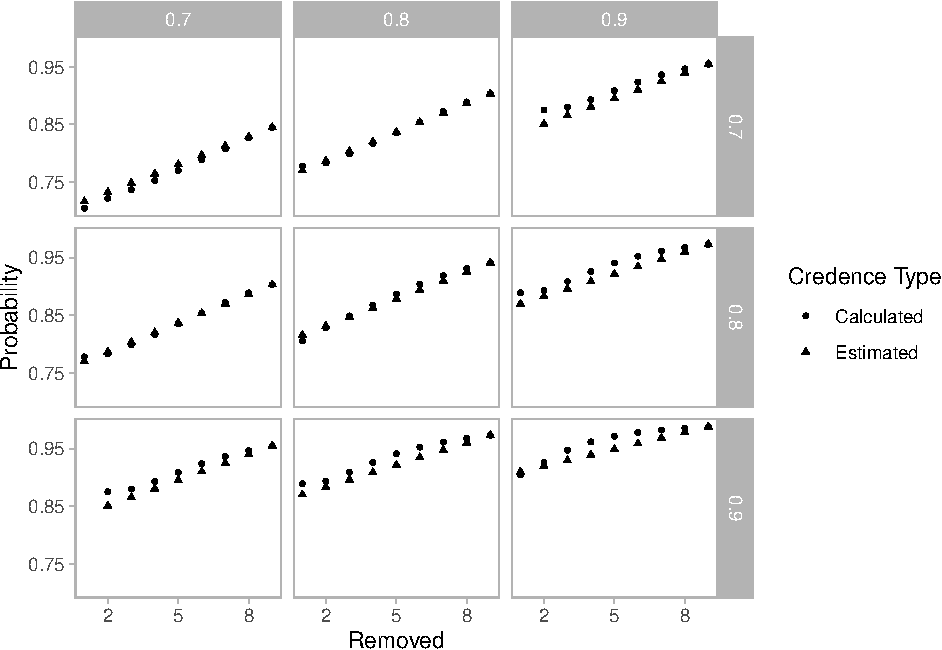
\includegraphics{mixing-experts-not-anon_files/figure-latex/unnamed-chunk-5-1.pdf}

That looks pretty good. There is a tiny bit of separation in the bottom
right panel, but otherwise the estimate tracks the calculated credences
pretty closely. Let's look at the middle of the graph.

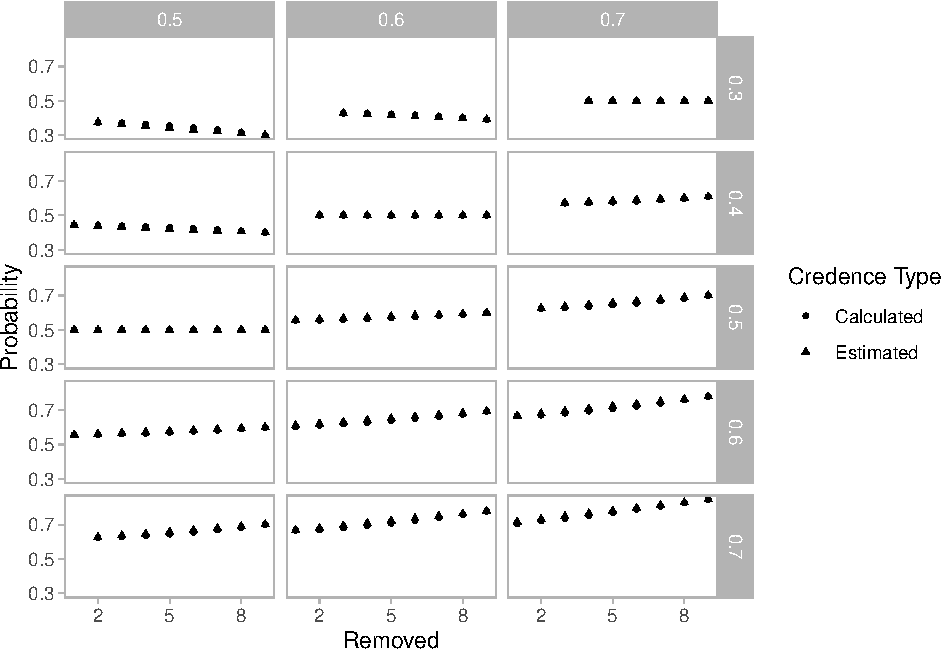
\includegraphics{mixing-experts-not-anon_files/figure-latex/unnamed-chunk-6-1.pdf}

And all through here the dots are overlapping. That's close enough. So
at least in this special case, the supra-Bayesian can produce an
estimate that is very close to the ideally calculated credence. So we
don't need to resort to pooling even as an approximation device.

But the simplifications here are dire. Here are six ways we might want
to generalise the model.

\begin{enumerate}
\def\labelenumi{\arabic{enumi}.}
\tightlist
\item
  Have the prior probabilities of \(p\) and \(\neg p\) vary.
\item
  Have more colors for the marbles, and have each expert announce
  credences over all the colors.
\item
  Have the person doing the merger be uncertain about \(k\).
\item
  Have the experts sample the jars they are given, not inspect them
  fully.
\item
  Have more than two experts.
\item
  Allow that some experts are more informed than others.
\end{enumerate}

The first two points are not that hard. I could produce a string of
graphs for different priors over the colors, or for more colors, and the
typical story is not that different to what we've seen so far. It just
gets messy because we have more degrees of freedom than is consistent
with a concise graphical display.

The next two points are harder. It's not that they are harder to come up
with the idea value. For any prior over \(k\), or sampling technique
that's available to the expert, it's pretty easy to write code to come
up with the optimal calculated credences. It's rather that the number of
degrees of freedom are so great that it gets a little harder to eyeball
how good any given approximation is. The big point is that the posterior
distribution of \(k\) will usually be different to the prior. In extreme
cases, the announced expert credences might rule out some hypotheses
about \(k\). So it won't just be a matter of calculating the values of
(9) for each value of \(k\), and averaging them out using the prior
probabilities of \(k\). There is a lot of possible future research here.

Having more than two experts raises both computational questions, like
what we've just discussed, and conceptual questions. Consider even what
happens when we go to three experts. Imagine the balls are numbered, and
say \(M_i\) is the proposition that ball \(i\) is numbered, and
\(J_{i, e}\) is that ball \(i\) is in the jar shown to expert \(e\). To
represent the degree of connectedness of one expert's evidence to the
other(s) in the two expert case, we really just need to specify one
variable: \(\Pr(J_{i, 1} | J_{i, 2} \wedge \neg M_i)\). But in the three
expert case, we need three variables to be specified.

\begin{itemize}
\tightlist
\item
  \(\Pr(J_{i, 1} | J_{i, 2} \wedge J_{i, 3} \wedge \neg M_i)\)
\item
  \(\Pr(J_{i, 1} | J_{i, 2} \wedge \neg J_{i, 3} \wedge \neg M_i)\)
\item
  \(\Pr(J_{i, 1} | \neg J_{i, 2} \wedge J_{i, 3} \wedge \neg M_i)\)
\end{itemize}

And if there are four experts, there are seven of these variables. And
this number grows exponentially as the number of experts rises.

The point is not just that the compututations of the ideal
supra-Bayesian credence require an exponentially increasing number of
inputs as the number of experts rises. It's that even thinking about how
to approximate this ideal calculation, we need a good way to
conceptualise this space whose dimensionality rises exponentially with
the number of experts in a way that lets us even think about what a good
approximation would look like. I don't have an answer to this; it feels
like a question for future research.

What I will try to make some headway on instead is the last question,
what happens if we do not assume the experts are just as well informed
as each other.

\hypertarget{case-three-differentially-informed-experts}{%
\section{Case Three: Differentially Informed
Experts}\label{case-three-differentially-informed-experts}}

In our last case, one expert is better informed than the other. Carmen
first fills the jar with the marked marble and 19 randomly chosen
unmarked marbles. She flips a coin to decide which expert to show this
jar to. They inspect the jar, and record their credence in \(p\) to the
nearest 0.1. (We'll come back very soon to why this is rounded.) Carmen
then removes 10 unmarked marbles from the jar, chosen at random, and
then shows it to the other expert. They inspect it, and come up with a
new credence in \(p\). Then both these recorded numbers are reported to
Player, without any indication about who saw the larger jar and who saw
the smaller one.

There is a weird thing in this setup in that one of the experts reports
something other than their precise credence. The reason I set up the
example this way is to make it impossible for the recipient of the
expert opinion to infer who saw the smaller jar. If they both reported
their actual credence, it would be possible for the recipient to be told
one of them has credence 0.75 in \(p\) and the other has credence 0.6.
And then it would be obvious that the hearer should have credence 0.6 in
\(p\), since that's the credence of the more informed person. So I made
the first person round to the nearest 0.1 to make it harder to make such
inferences.

Given all that setup we can work out what Player's credence in \(p\)
should be given the two announcements. (I'm rounding to three decimal
places to save space.I'm leaving off the cases where one or other party
announces an extremal credence - the hearer agrees with those credences,
at least to three decimal places. And the `NA' values are where it is
impossible given the setup for those to be the announced values.)

\begin{tabular}{rrrrrrrrrr}
\toprule
Ivy/Zack & 0.1 & 0.2 & 0.3 & 0.4 & 0.5 & 0.6 & 0.7 & 0.8 & 0.9\\
\midrule
0.1 & 0.100 & 0.103 & 0.100 & 0.100 & 0.100 & 0.100 & NA & NA & NA\\
0.2 & 0.103 & 0.200 & 0.208 & 0.203 & 0.202 & 0.200 & NA & NA & NA\\
0.3 & 0.100 & 0.208 & 0.300 & 0.320 & 0.325 & 0.348 & 0.500 & NA & NA\\
0.4 & 0.100 & 0.203 & 0.320 & 0.400 & 0.439 & 0.500 & 0.652 & 0.800 & 0.900\\
0.5 & 0.100 & 0.202 & 0.325 & 0.439 & 0.500 & 0.561 & 0.675 & 0.798 & 0.900\\
0.6 & 0.100 & 0.200 & 0.348 & 0.500 & 0.561 & 0.600 & 0.680 & 0.797 & 0.900\\
0.7 & NA & NA & 0.500 & 0.652 & 0.675 & 0.680 & 0.700 & 0.792 & 0.900\\
0.8 & NA & NA & NA & 0.800 & 0.798 & 0.797 & 0.792 & 0.800 & 0.897\\
0.9 & NA & NA & NA & 0.900 & 0.900 & 0.900 & 0.900 & 0.897 & 0.900\\
\bottomrule
\end{tabular}

And a striking thing about this table is how close it comes to verifying
a strong form of what \protect\hyperlink{ref-Levinstein2015}{Levinstein}
(\protect\hyperlink{ref-Levinstein2015}{2015}) calls Thrasymachus'
Principle. The hearer defers to the expert with the strongest view,
i.e., the view that's furthest from the prior. In contemporary terms,
the hearer listens to the expert with the hottest take. It isn't an
unvarnished form of that. When one says 0.5 and the other says 0.6 you
end up with 0.561, not 0.6. But that's in large part because there's a
good chance that the person who said 0.6 was merely rounding up as the
result of a coin flip. In general, the rule in this case is find the
expert credence that is furthest from the prior, and adopt it.

There is a reason that a case like this should follow Thrasymachus'
Principle. If the experts are rational, hotter takes should correspond
to stronger evidence. And while it isn't impossible for the person with
more evidence to have in a sense weaker evidence, the extra evidence may
be full of defeaters for the first obtained evidence, it is pretty
unlikely. In general, if someone is worthy of deference, and they have a
strong view, they have strong evidence. If someone else has a weaker
view, i.e., a view closer to the prior, the best explanation is that
they simply don't have the evidence that the person with stronger view
does.

So again, we shouldn't pool the opinions in any interesting sense. The
table shows the optimal response by supra-Bayesian lights. And the
simple approximation is, ``When one expert has clearly stronger views,
listen to them. Otherwise take the geometric mean.''

\hypertarget{summary}{%
\section{Summary}\label{summary}}

Let's take stock of what's been covered so far.

\begin{itemize}
\tightlist
\item
  I've argued against all three uses of pooling answers to the question
  of how to merge expert opinions. Sometimes the pooling answer is
  clearly wrong, often it won't be a good constraint on priors, and
  there are better ways to approximate the correct supra-Bayesian
  answer.
\item
  I've connected supra-Bayesianism to some familiar positions in
  epistemology, the view on testimony in
  \protect\hyperlink{ref-Jackson1987}{Jackson}
  (\protect\hyperlink{ref-Jackson1987}{1987}) and the view on
  disagreement in \protect\hyperlink{ref-Lackey2010-LACWSW}{Lackey}
  (\protect\hyperlink{ref-Lackey2010-LACWSW}{2010}).
\item
  I've shown that if you take that approach, that conditionalising on
  someone else's credence is just conditionalising on the fact that they
  have evidence that rationalises such a credence by their lights, then
  the principle \protect\hyperlink{ref-EaswaranEtAl2016}{Easwaran et
  al.} (\protect\hyperlink{ref-EaswaranEtAl2016}{2016}) recommend for
  updating on the credences of others follows directly from the
  assumptions that each expert is independently worthy of deference, and
  the evidence the experts have is conditionally independent.
\item
  I've developed a toy example that lets us think about cases where the
  hearer doesn't know which parts of the evidence are in common, but
  does know how much is in common.
\item
  And I've shown that in that case, the correct supra-Bayesian answer is
  nicely approximated by a linear average of two familiar formulas.
\item
  I developed a toy example that lets us think about the case where one
  expert is known to be more informed, but we aren't sure which it is.
\item
  And in that case I showed that what
  \protect\hyperlink{ref-Levinstein2015}{Levinstein}
  (\protect\hyperlink{ref-Levinstein2015}{2015}) calls Thrasymachus'
  Principle is approximately right; we should defer to the `stronger,'
  i.e., more opinionated, expert.
\end{itemize}

At the end of section 2 I mentioned six ways in which we might make the
model even more general. This is very much not meant to be the last
word. But I suspect these kinds of examples can be used to provide
useful approximations, or guides, to real life situations where we know
something about the relationship between the experts. The general lesson
is that by looking at toy cases, we can provide practical advice for how
to emulate, or at least approximate, the supra-Bayesian approach for
merging expert opinion. And this advice will be better than the advice
that anyone who ignores the relationship between the experts can offer.

But there is one last kind of relationship between experts that I
haven't made any progress on modeling, and it is a big one. What should
we say about cases where the experts know each others credences? This is
an old and, to my mind, open question. For reasons that trace back to
\protect\hyperlink{ref-Aumann1976}{Aumann}
(\protect\hyperlink{ref-Aumann1976}{1976}), in anything like the kind of
model I've used here, if the experts know each other's credences, they
have to agree. And someone who knows both credences should agree with
them. But the real world obviously contains experts who do agree to
disagree. What to say about those cases is the biggest open questions
around here, and I'm not sure whether this approach can help.
\protect\hyperlink{ref-Gallow2018}{Gallow}
(\protect\hyperlink{ref-Gallow2018}{2018}) ends his paper by raising
doubts about whether it is rational to be disposed to defer to two
different experts. I'm not worried about that in general; I've described
three very different kinds of cases where it is rational. But I suspect
one could not be rationally disposed to defer to two experts who one
knows are themselves disposed to agree to disagree. That, however, is a
story for another paper. This paper has described a number of cases
where the hearer knows something the experts doesn't know: namely what
other experts think. And it has described both precise and approximate
answers for what to do in those interesting cases.

\hypertarget{references}{%
\subsection*{References}\label{references}}
\addcontentsline{toc}{subsection}{References}

\hypertarget{refs}{}
\begin{CSLReferences}{1}{0}
\leavevmode\hypertarget{ref-Aumann1976}{}%
Aumann, Robert J. 1976. {``Agreeing to Disagree.''} \emph{The Annals of
Statistics} 4 (6): 1236--39.
\url{https://doi.org/10.1214/aos/1176343654}.

\leavevmode\hypertarget{ref-BaccelliStewart2021}{}%
Baccelli, Jean, and Rush T. Stewart. 2021. {``Support for Geometric
Pooling.''} \emph{Review of Symbolic Logic} forthcoming.
\url{https://doi.org/doi:10.1017/S1755020320000416}.

\leavevmode\hypertarget{ref-Bradley2017}{}%
Bradley, Richard. 2017. {``Learning from Others: Conditioning Versus
Averaging.''} \emph{Theory and Decision} 85 (1): 5--20.
\url{https://doi.org/10.1007/s11238-017-9615-y}.

\leavevmode\hypertarget{ref-EaswaranEtAl2016}{}%
Easwaran, Kenny, Luke Fenton-Glynn, Christopher Hitchcock, and Joel D.
Velasco. 2016. {``Updating on the Credences of Others: Disagreement,
Agreement, and Synergy.''} \emph{Philosophers' Imprint} 16 (11): 1--39.

\leavevmode\hypertarget{ref-Elga2007}{}%
Elga, Adam. 2007. {``Reflection and Disagreement.''} \emph{No{û}s} 41
(3): 478--502. \url{https://doi.org/10.1111/j.1468-0068.2007.00656.x}.

\leavevmode\hypertarget{ref-Gallow2018}{}%
Gallow, J. 2018. {``No One Can Serve Two Epistemic Masters.''}
\emph{Philosophical Studies} 175 (10): 2389--98.
\url{https://doi.org/10.1007/s11098-017-0964-8}.

\leavevmode\hypertarget{ref-Jackson1987}{}%
Jackson, Frank. 1987. \emph{Conditionals}. Blackwell: Oxford.

\leavevmode\hypertarget{ref-Lackey2010-LACWSW}{}%
Lackey, Jennifer. 2010. {``What Should We Do When We Disagree.''}
\emph{Oxford Studies in Epistemology} 3: 274--93.

\leavevmode\hypertarget{ref-Levinstein2015}{}%
Levinstein, Benjamin Anders. 2015. {``With All Due Respect: The
Macro-Epistemology of Disagreement.''} \emph{Philosophers' Imprint} 15
(13): 1--20.

\leavevmode\hypertarget{ref-RussellEtAl2015}{}%
Russell, Jeffrey Sanford, John Hawthorne, and Lara Buchak. 2015.
{``Groupthink.''} \emph{Philosophical Studies} 172 (5): 1287--1309.
\url{https://doi.org/10.1007/s11098-014-0350-8}.

\end{CSLReferences}

\end{document}
